% !TEX root = ./document.tex

\documentclass[a4paper, spanish]{article}

\usepackage{mystyle}
\usepackage{myvars}

\begin{document}

  \maketitle

  \begin{itemize}
    \item \textbf{Archivo}: \texttt{tuberculo.sf3}
    \item \textbf{Serie}: Número de casos registrados semanalmente de tuberculosis respiratoria en España, entre los años $1982$ y $1991$ (el primer dato corresponde al número de casos registrados desde el \emph{$1$ de Enero de $1982$} al \emph{$7$ de Enero de $1982$}).
    \begin{itemize}
      \item $\{X_t\}$ Serie Original.
      \item $\{Y_t\}$ Serie del número de casos en periodos de cuatro semanas sucesivos.
    \end{itemize}
  \end{itemize}

  \section{Describir estas dos series ($\{Y_t\}$ puede crearse con el \texttt{proc expand} de \emph{SAS}), indicando claramente para cada una de ellas qué frecuencias elegiríais a priori para ajustar un modelo con tendencia polinómica más ondas.}
  \label{sec:a}

    \paragraph{}
    [TODO]

    \subsection{Serie Semanal: $\{X_t\}$}

      \paragraph{}
      [TODO]

      \begin{listing}[htb!]
        \centering
        \inputminted{SAS}{./res/code/a-01-data.sas}
        \caption{Generación del conjunto de datos \texttt{EJ2.SEMANAL}}
        \label{code:a_data}
      \end{listing}

      \paragraph{}
      [TODO]

      \begin{figure}[htb!]
        \centering
        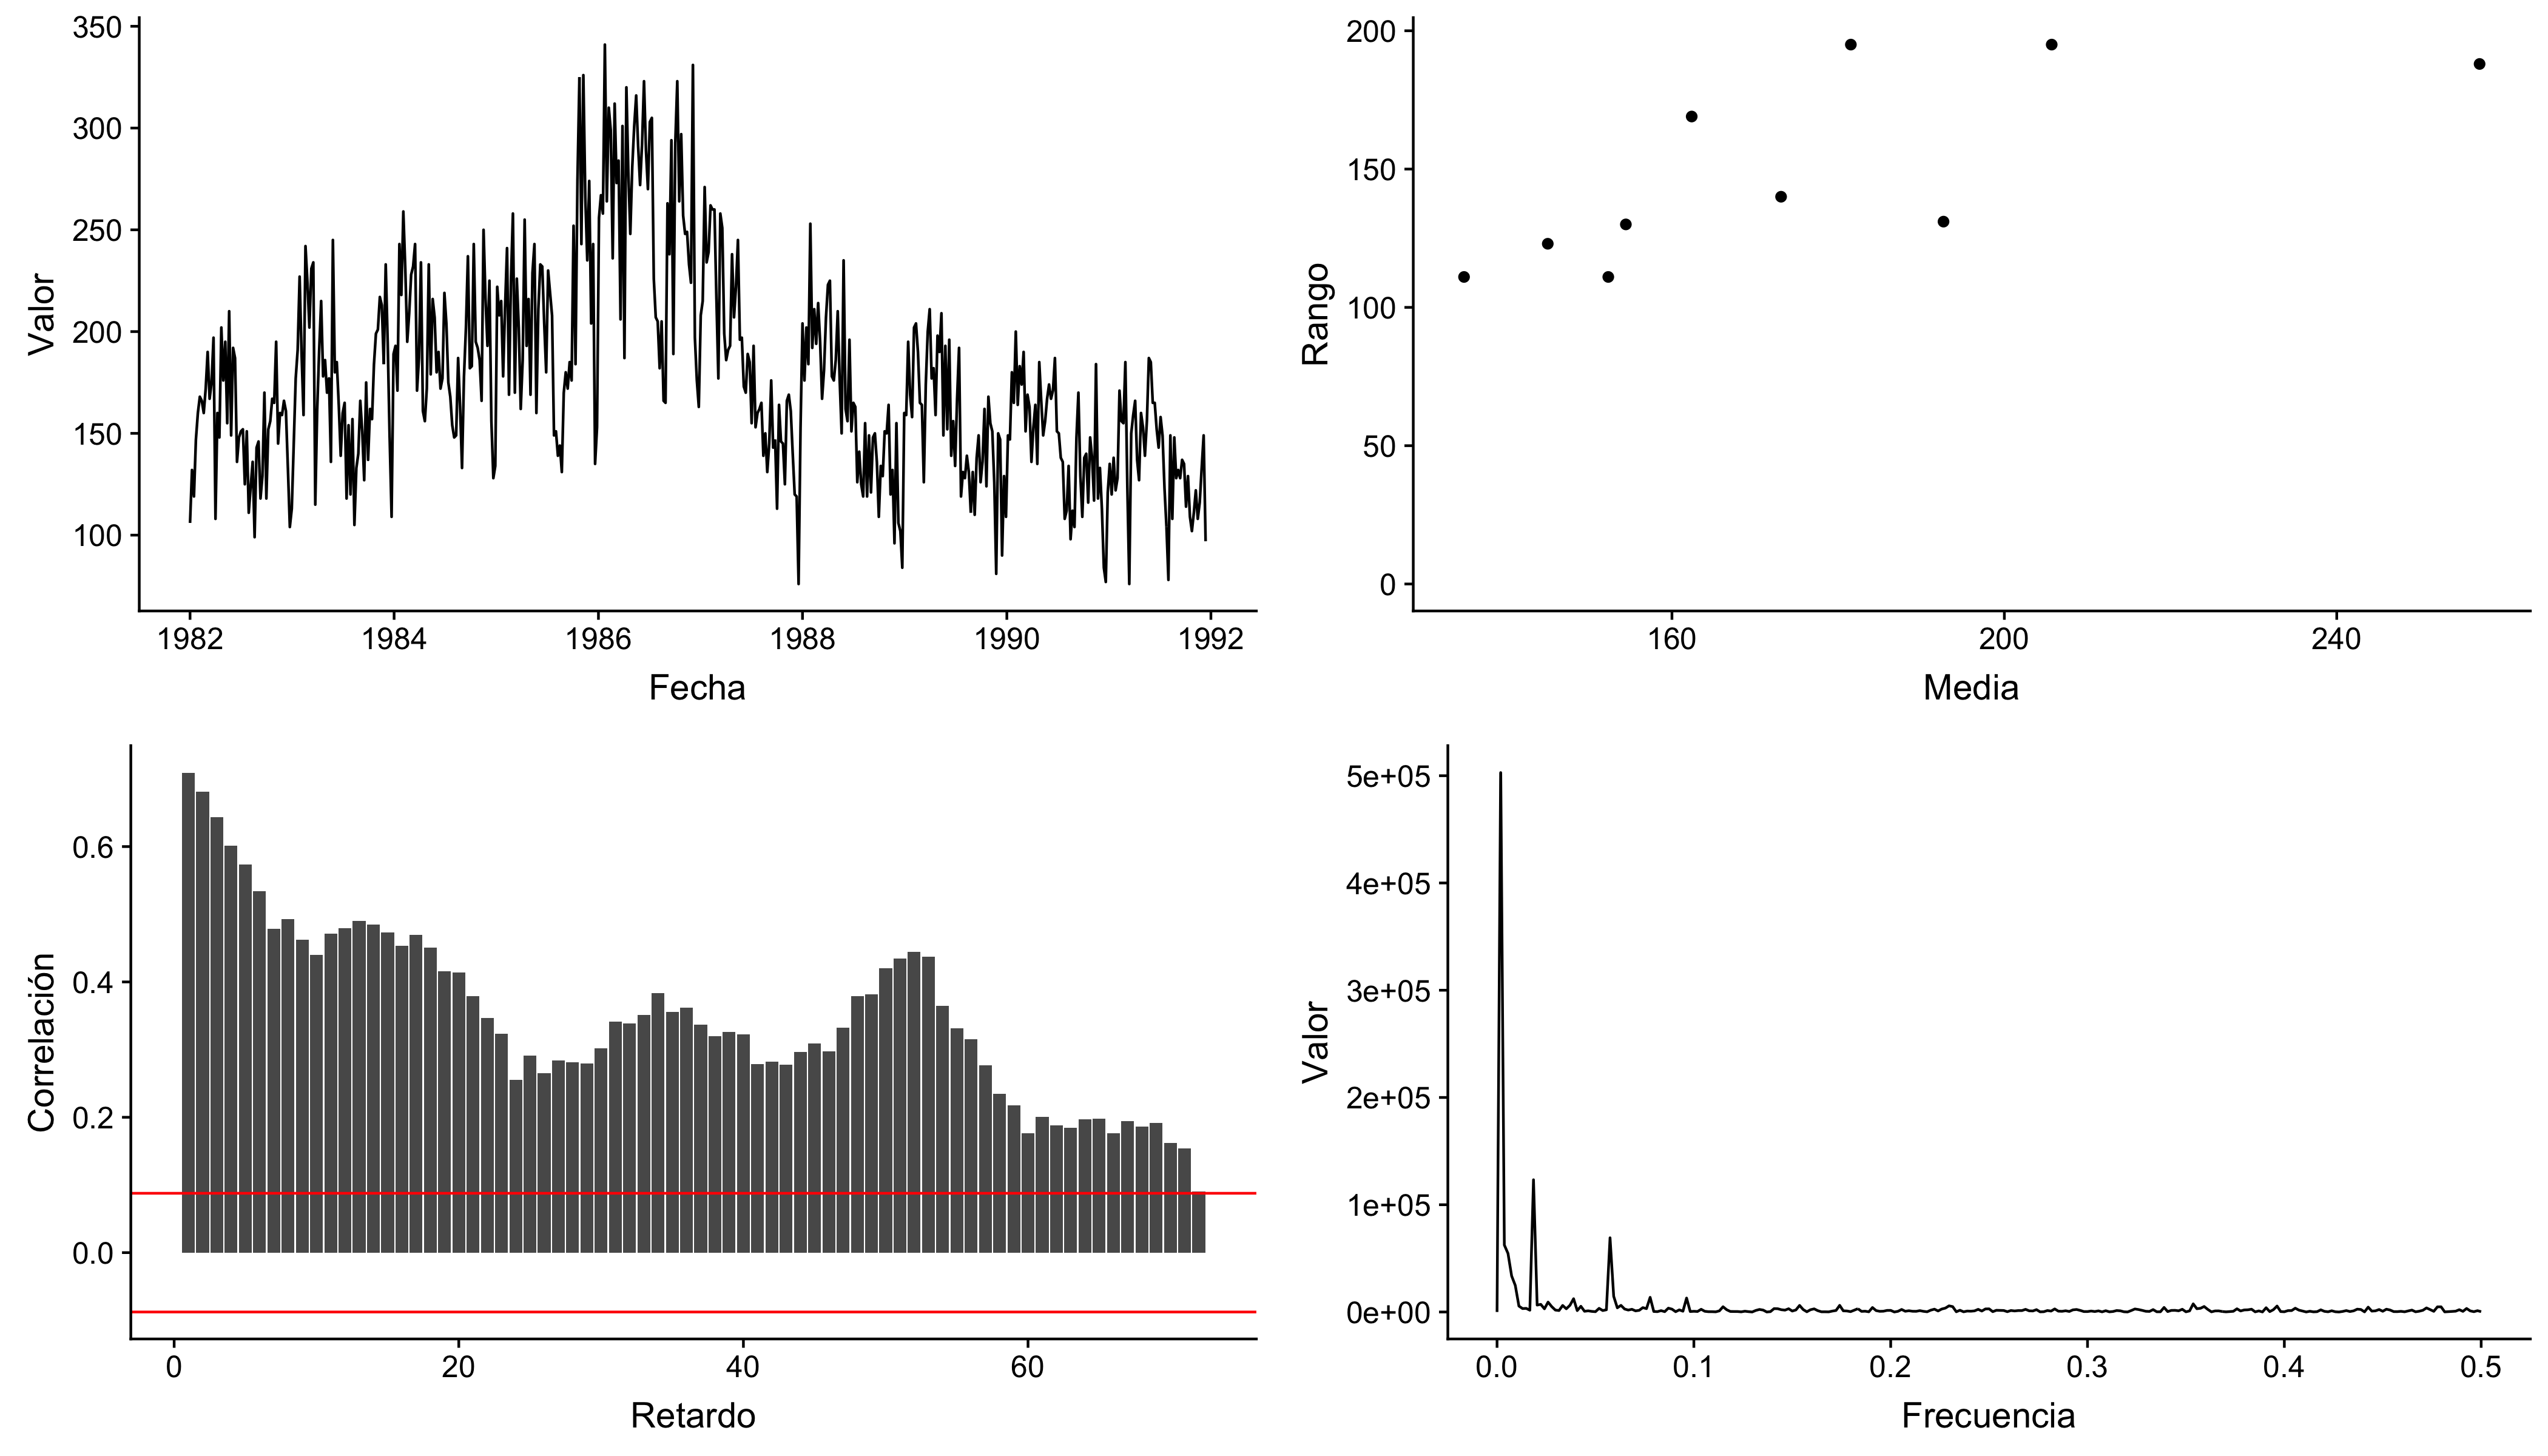
\includegraphics[width=.75\linewidth]{semanal}
        \caption{Gráfico de la serie, gráfico de dispersión \emph{rango-media}, \emph{correlograma} y \emph{periodograma} del conjunto de datos \texttt{EJ2.SEMANAL}}
        \label{img:semanal}
      \end{figure}

      \paragraph{}
      [TODO]

      \begin{figure}[htb!]
        \centering
        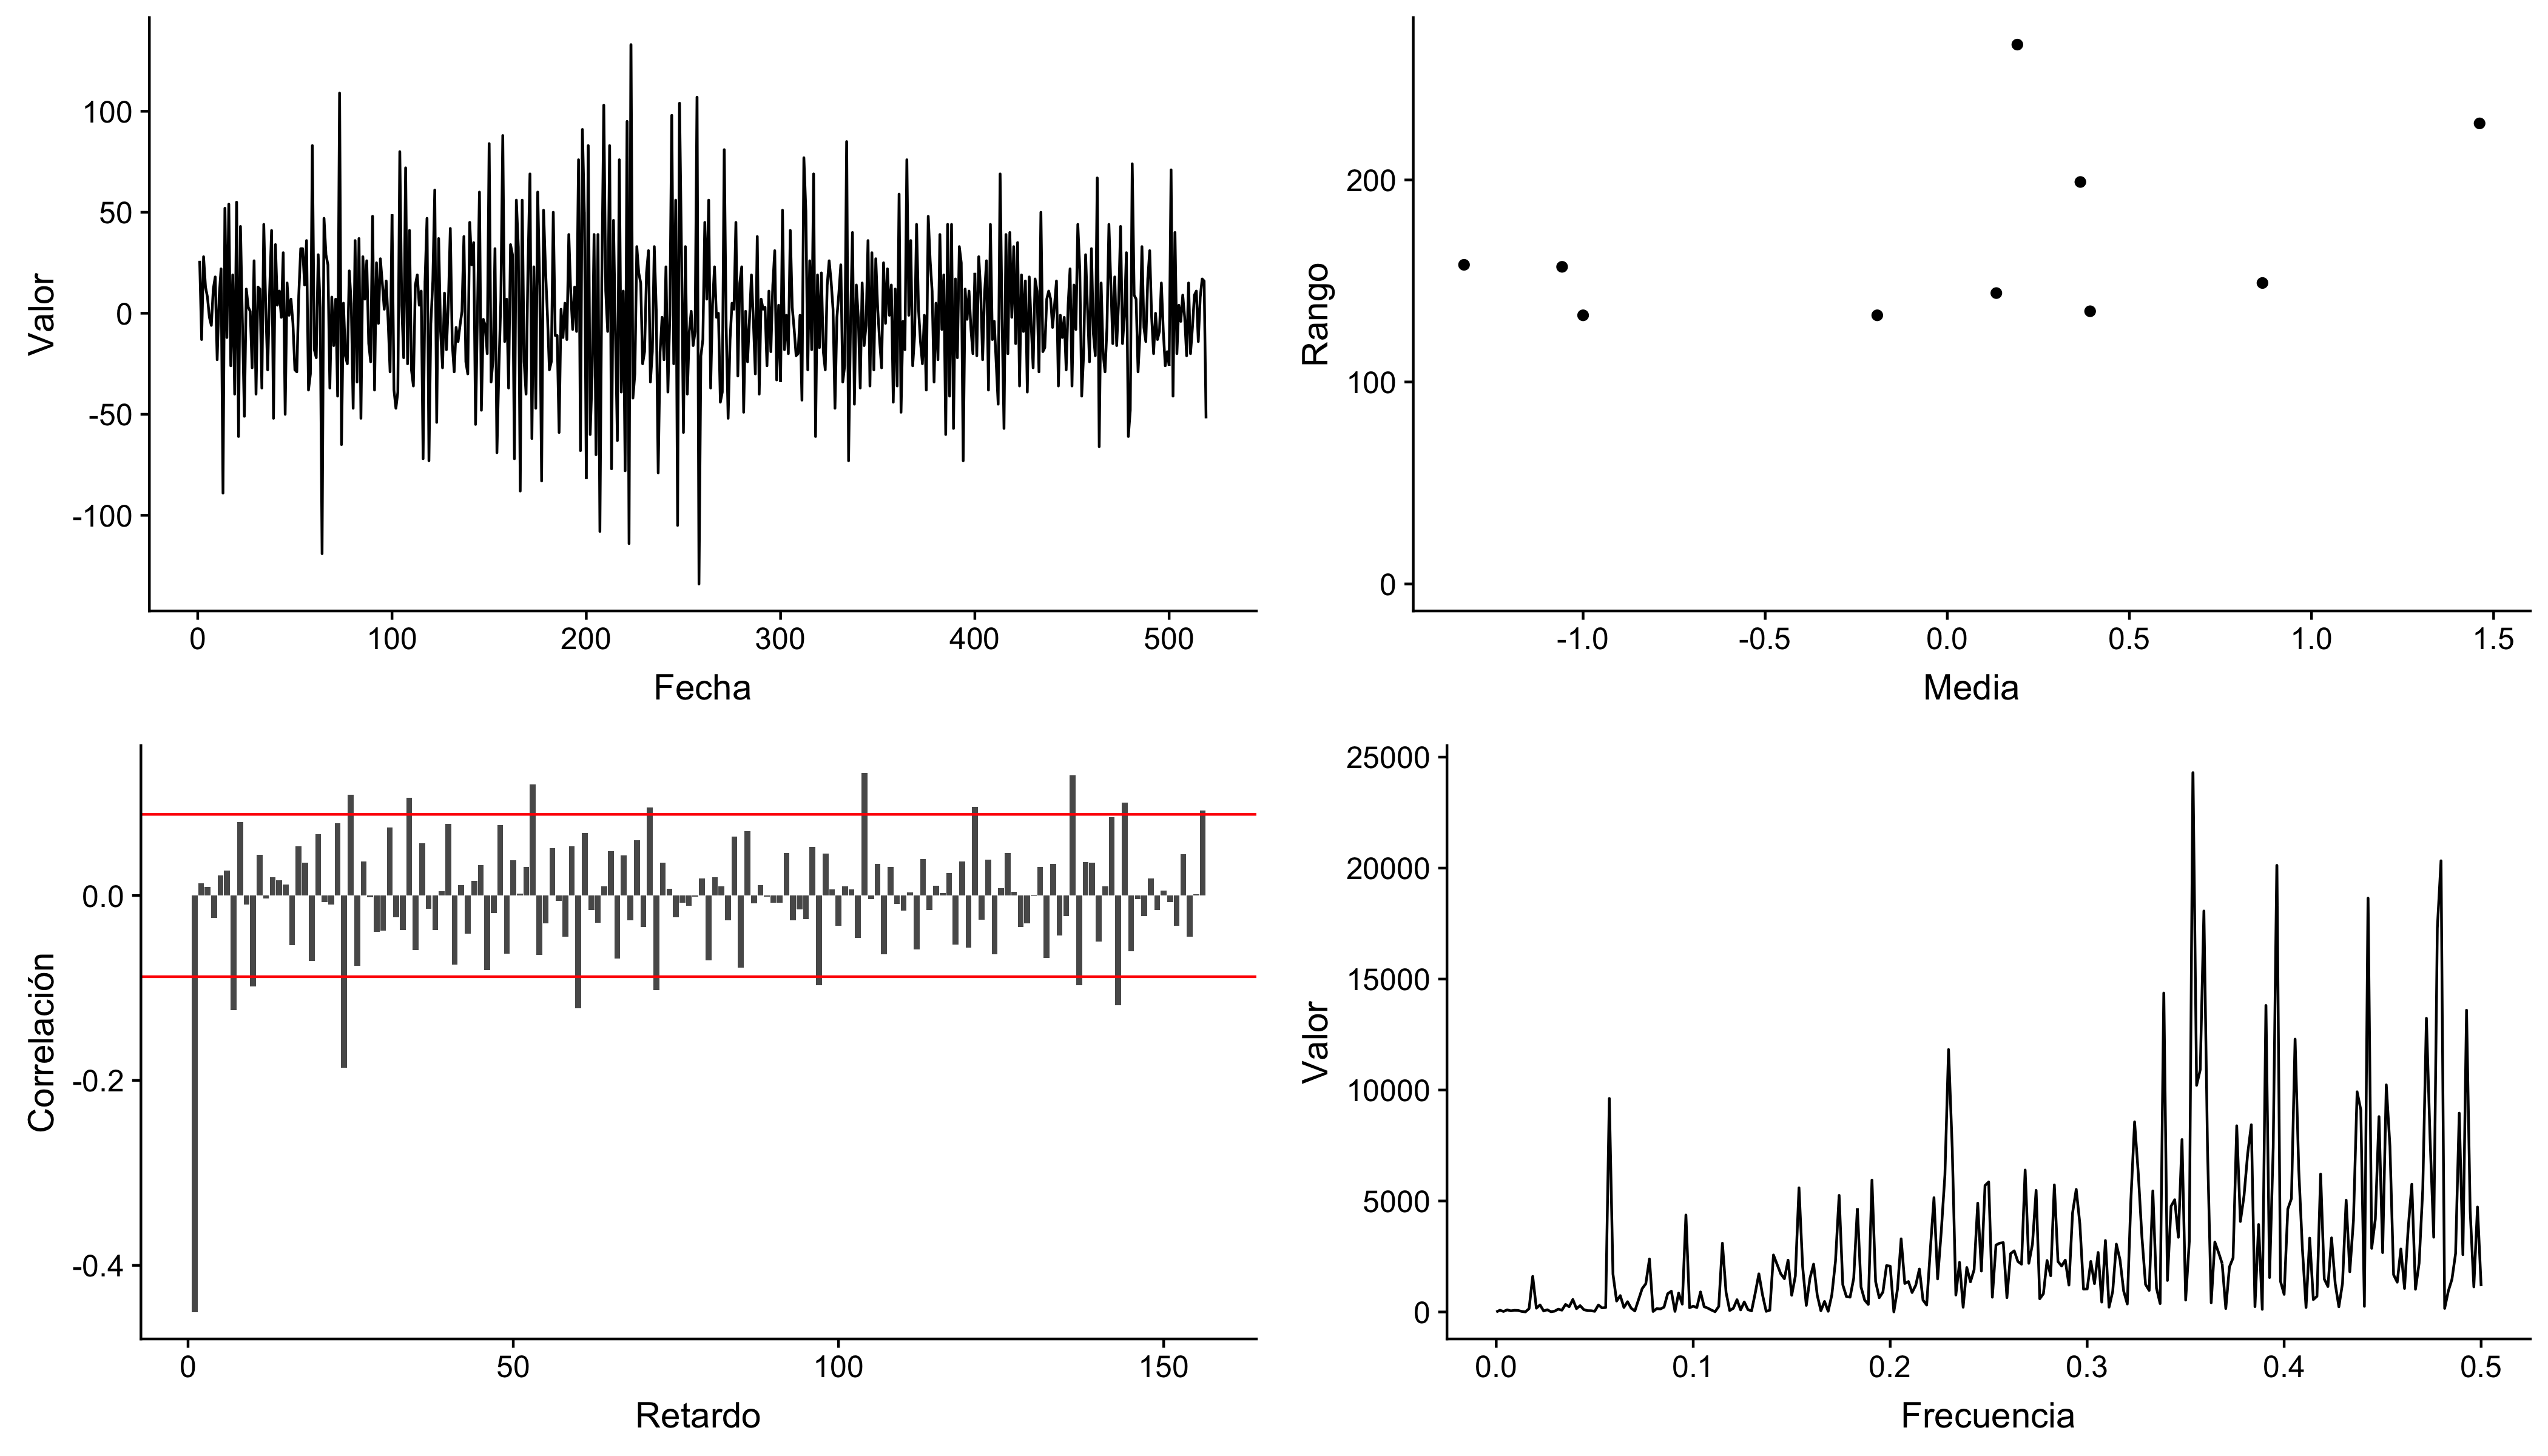
\includegraphics[width=.75\linewidth]{semanal-diff}
        \caption{Gráfico de la serie, gráfico de dispersión \emph{rango-media}, \emph{correlograma} y \emph{periodograma} del conjunto de datos \texttt{EJ2.SEMANAL} tras aplicar una diferenciación de primer orden.}
        \label{img:semanal_diff}
      \end{figure}

      \paragraph{}
      [TODO]

    \subsection{Serie  4 semanas: $\{Y_t\}$}

      \paragraph{}
      [TODO]

      \begin{listing}[htb!]
        \centering
        \inputminted{SAS}{./res/code/a-02-expand.sas}
        \caption{Generación del conjunto de datos \texttt{EJ2.SEMANAL4} a partir de \texttt{EJ2.SEMANAL}}
        \label{code:a_expand}
      \end{listing}

      \paragraph{}
      [TODO]

      \begin{figure}[htb!]
        \centering
        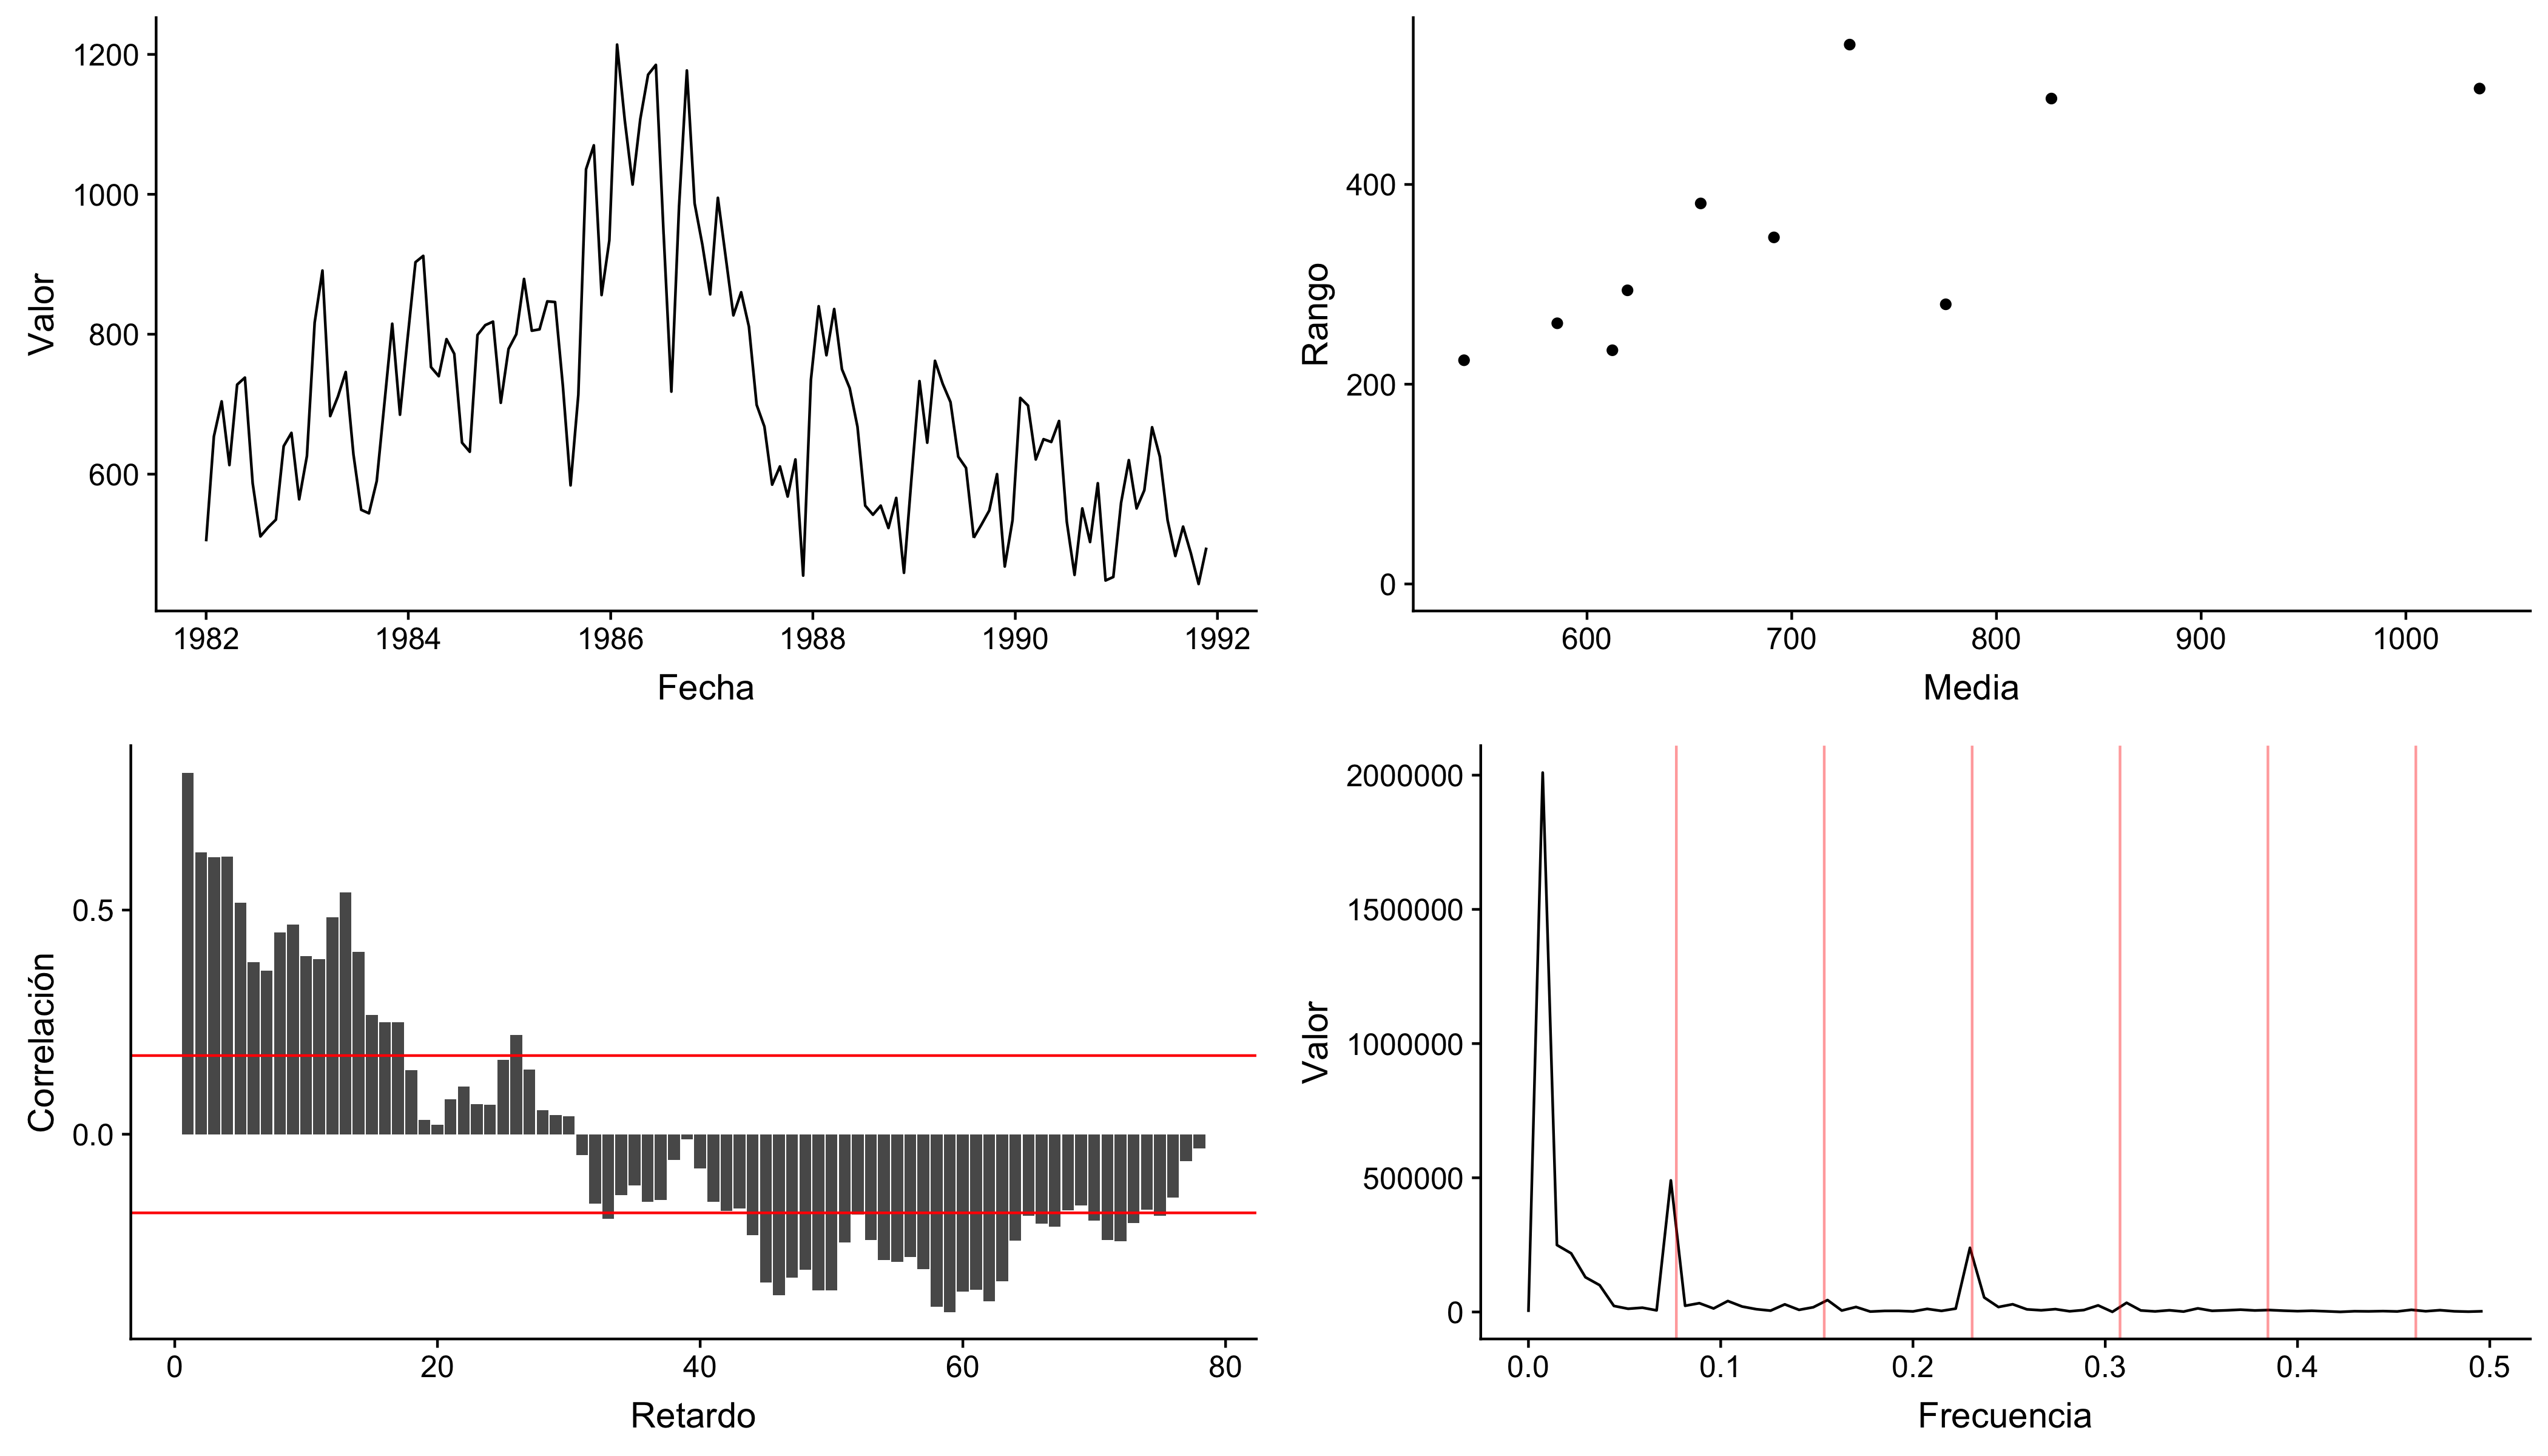
\includegraphics[width=.75\linewidth]{semanal4}
        \caption{Gráfico de la serie, gráfico de dispersión \emph{rango-media}, \emph{correlograma} y \emph{periodograma} del conjunto de datos \texttt{EJ2.SEMANAL4}}
        \label{img:semanal4}
      \end{figure}

      \paragraph{}
      [TODO]

      \begin{figure}[htb!]
        \centering
        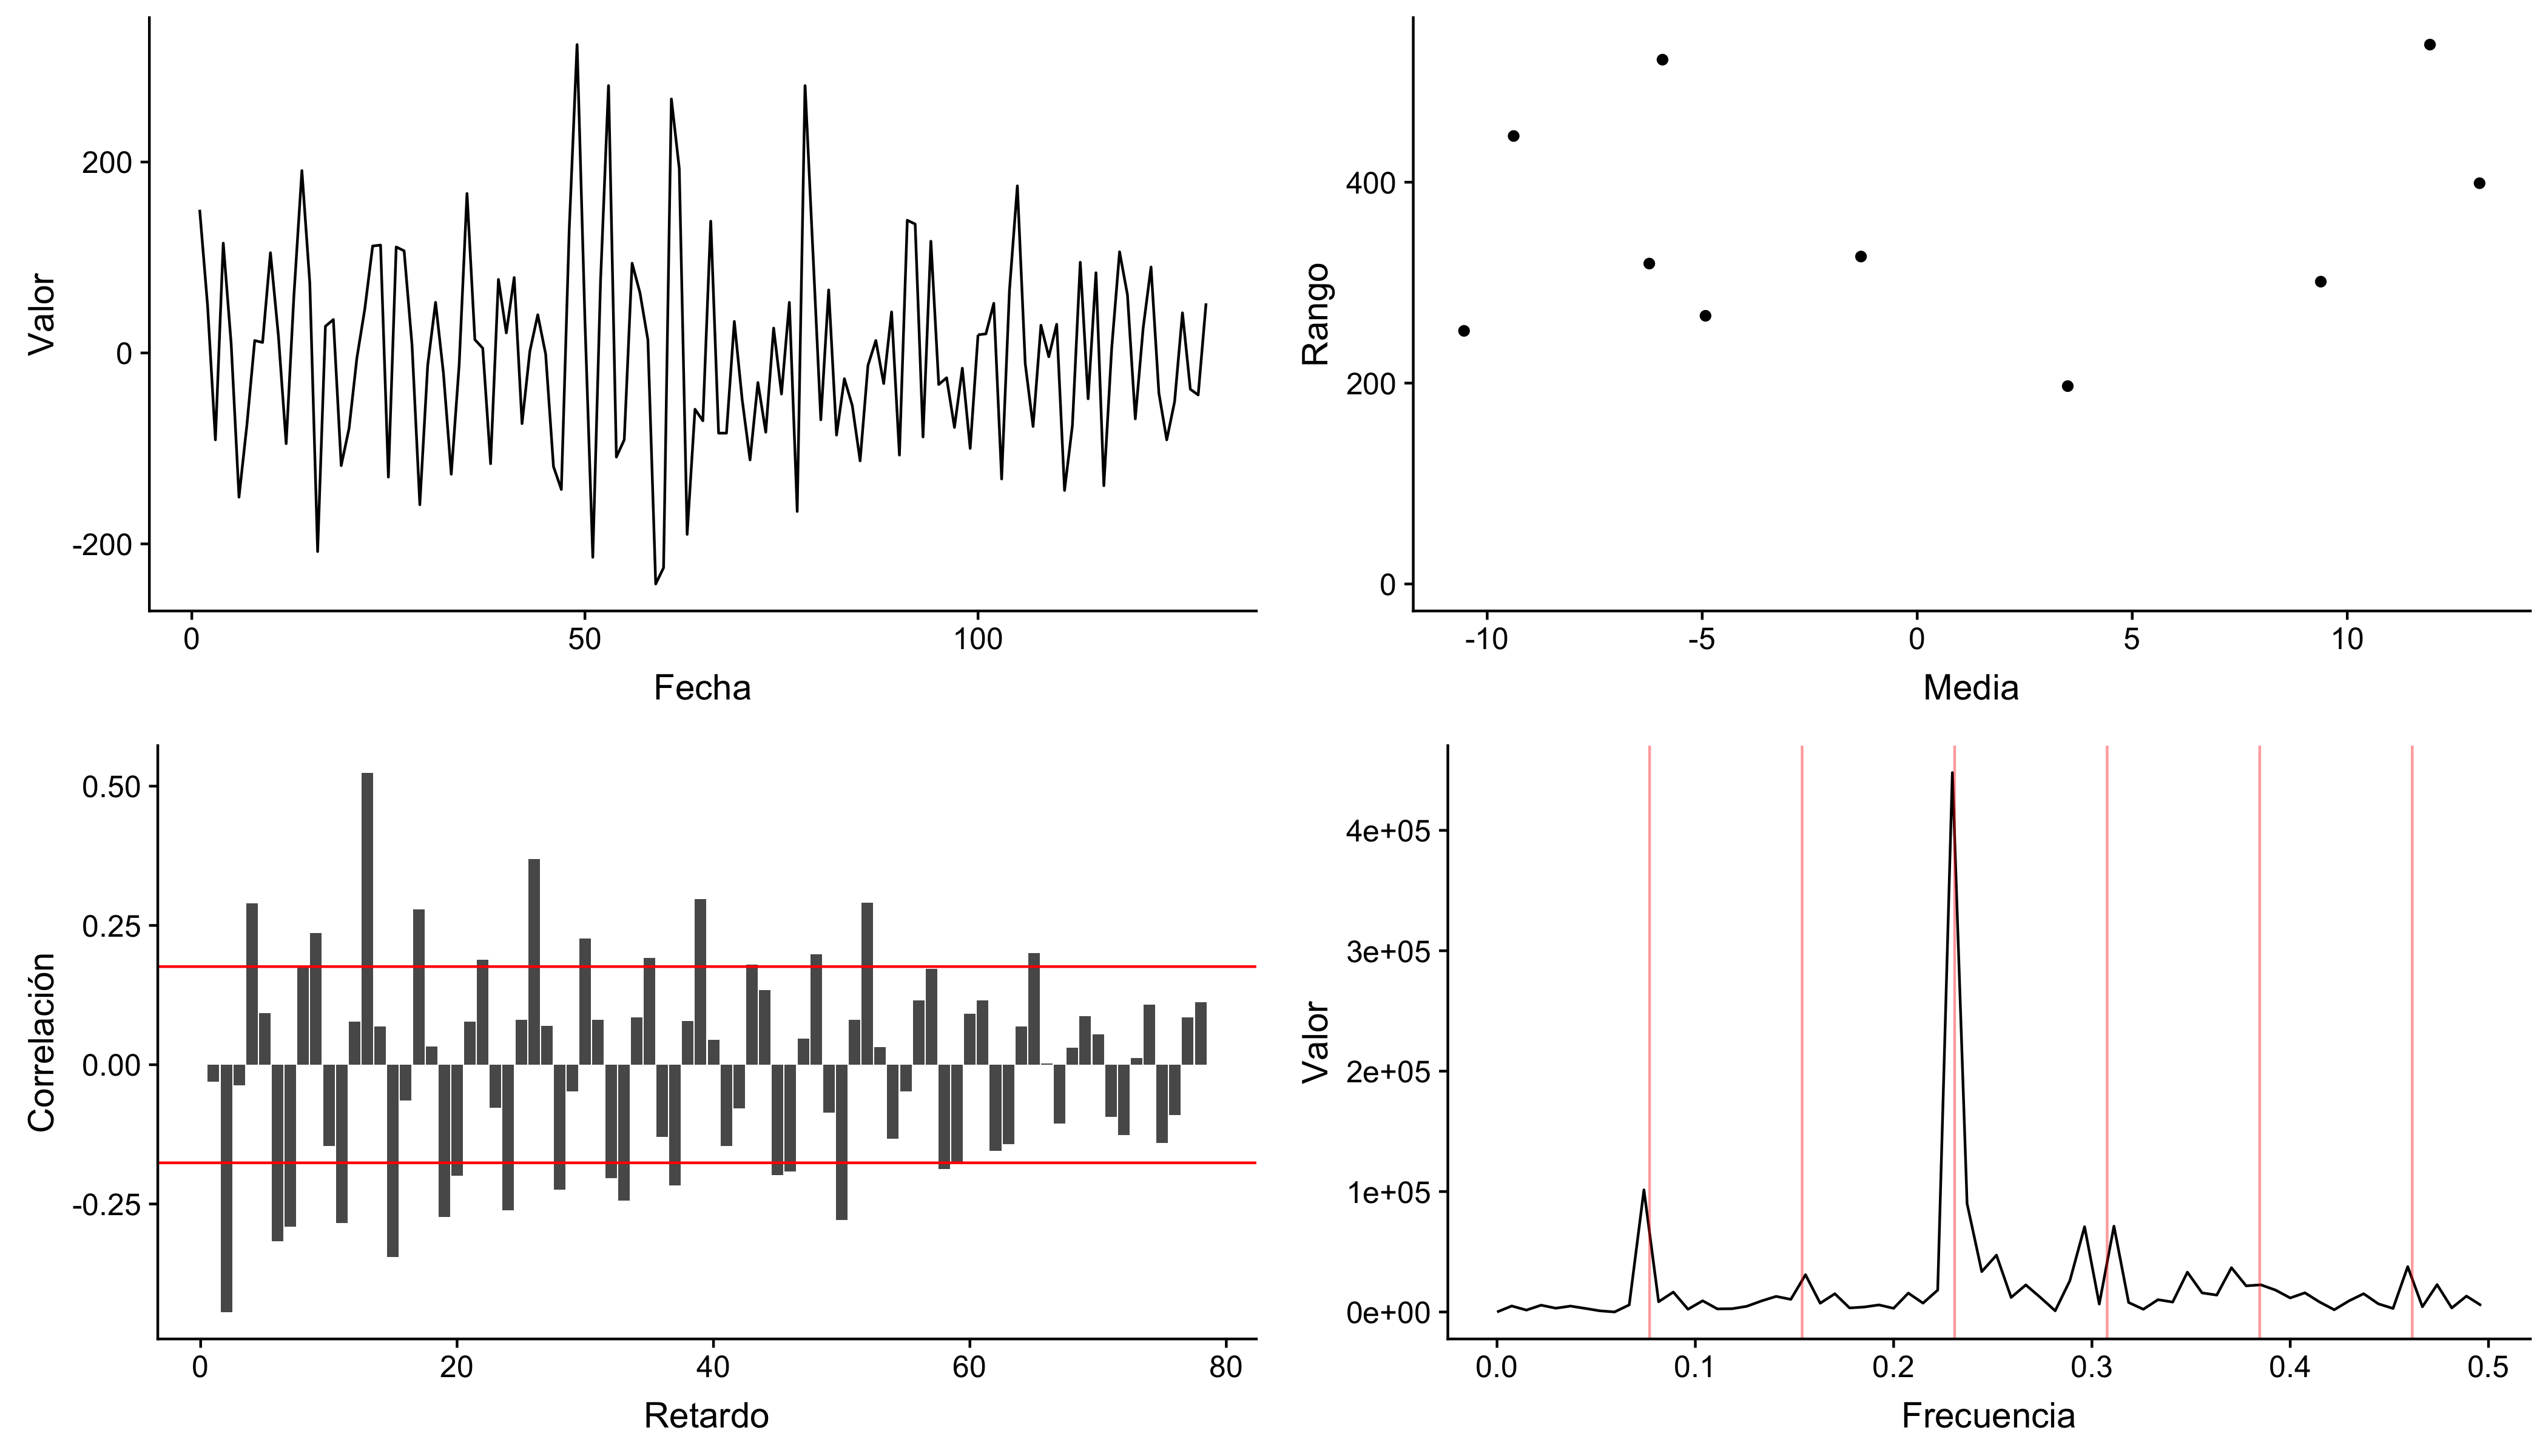
\includegraphics[width=.75\linewidth]{semanal4-diff}
        \caption{Gráfico de la serie, gráfico de dispersión \emph{rango-media}, \emph{correlograma} y \emph{periodograma} del conjunto de datos \texttt{EJ2.SEMANAL4} tras aplicar una diferenciación de primer orden.}
        \label{img:semanal4_diff}
      \end{figure}

      \paragraph{}
      [TODO]

    \paragraph{}
    [TODO]

  \section{Ajustar por suavizado exponencial, con el \texttt{proc esm}, los tres modelos que se consideren más apropiados para la serie $\{Y_t\}$ y comprobar su adecuación.}
  \label{sec:b}

    \paragraph{}
    Tras realizar un exhaustivo análisis de todas las diferentes posibilidades de ajuste por suavizado exponencial elegimos el \textit{seasonal exponential smoothing}, el \textit{suavizado de Winters multiplicativo} y el \textit{aditivo}, ya que son los tres que incorporarán la estacionalidad de la serie.

    \subsection{Suavizado Exponencial con Estacionalidad}

      \paragraph{}
      [TODO]

      \begin{listing}[htb!]
        \centering
        \inputminted{SAS}{./res/code/b-01-esm-seasonal.sas}
        \caption{Código fuente para el ajuste de un modelo de \emph{Suavizado Exponencial con Estacionalidad} sobre el conjunto de datos \texttt{EJ2.SEMANAL4}}
        \label{code:b_seasonal_esm}
      \end{listing}

      \paragraph{}
      [TODO]

      \paragraph{}
      Para comenzar explicaremos el modelo SES en el que mediante la tabla de los estimadores del parámetro y la significancia de dicho test.

      \begin{table}[htb!]
        \centering
        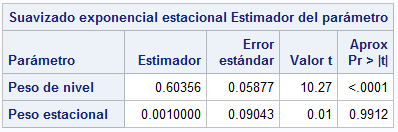
\includegraphics[width=0.75\textwidth]{PvalorSeasonal}
        \caption{Significancia para el modelo de \emph{Suavizado Exponencial con Estacionalidad} sobre el conjunto de datos \texttt{EJ2.SEMANAL4}}
        \label{table:b_seasonal_significance}
      \end{table}

      \paragraph{}
      Observamos que para la constante de suavizado estacional no se rechaza su significancia a cualquier nivel ya que el pvalor es 0.99.

      \paragraph{}
      En cambio, si se rechazará para la constante de suavizado para la media, donde el pvalor es $<0.001$. Será conveniente diferenciar ya que el estimador estacional es cercano a 0. A continuación adjuntamos el gráfico del ACF de residuales:

      \begin{figure}[htb!]
        \centering
        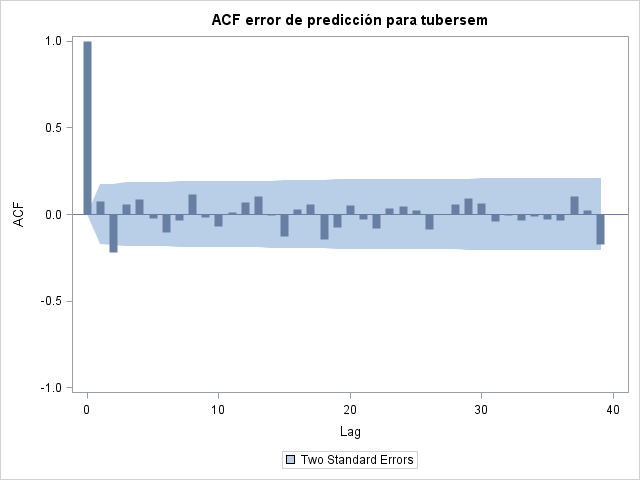
\includegraphics[width=0.75\textwidth]{ErrorACFPlot_SEASONAL}
        \caption{Gráfico de autocorrelaciones (correlograma) para los residuales del modelo de \emph{Suavizado Exponencial con Estacionalidad} sobre el conjunto de datos \texttt{EJ2.SEMANAL4}}
        \label{img:b_seasonal_residuals_correlogram}
      \end{figure}

      \paragraph{}
      Observamos como dicho modelo ofrece dudas sobre su validación ya que para el retardo 2 la autocorrelación es muy alta. El retardo 1 no es muy alto, no resultará perjudicial para el modelo. Los retardos estacionales(cada 13) no son notables por lo que es bueno para la validación.

      \begin{figure}[htb!]
        \centering
        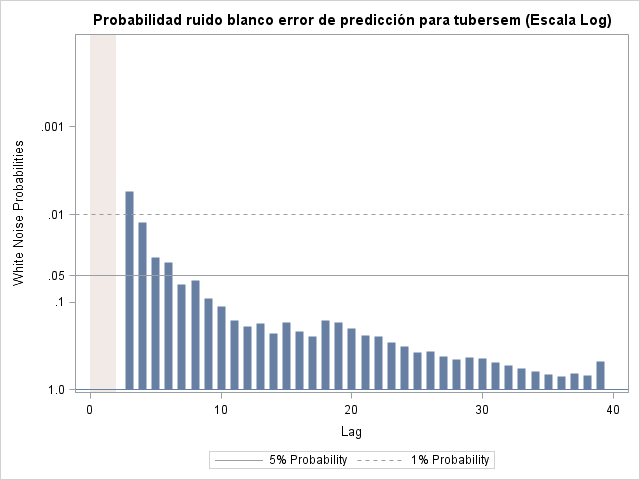
\includegraphics[width=0.75\textwidth]{ErrorWhiteNoiseLogProbPlot_SEASONAL}
        \caption{Gráfico sobre el contraste de ruido blanco para los residuales del modelo de \emph{Suavizado Exponencial con Estacionalidad} sobre el conjunto de datos \texttt{EJ2.SEMANAL4}}
        \label{img:b_seasonal_test_white_noise}
      \end{figure}

      \paragraph{}
      Vemos en la gráfica que el test de que las correlaciones sean cero se rechaza para los 4 primeros retardos a nivel 0.05. Esto es indeseable para validar el modelo puesto que no podemos asegurar que sea ruido blanco, que es lo que se busca.

      \paragraph{}
      A continuación, pasamos a realizar el ajuste del modelo aditivo de Winter.

    \subsection{Winter Aditivo}

      \paragraph{}
      [TODO]

      \begin{listing}[htb!]
        \centering
        \inputminted{SAS}{./res/code/b-01-esm-winteradd.sas}
        \caption{Código fuente para el ajuste de un modelo de \emph{Winter Aditivo} sobre el conjunto de datos \texttt{EJ2.SEMANAL4}}
        \label{code:b_winter_additive_esm}
      \end{listing}

      \paragraph{}
      [TODO]

      \begin{table}[htb!]
        \centering
        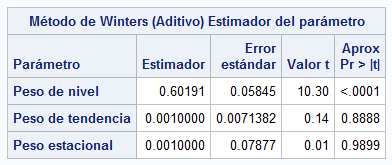
\includegraphics[width=0.75\textwidth]{TablaADD}
        \caption{Significancia para el modelo de \emph{Winter Aditivo} sobre el conjunto de datos \texttt{EJ2.SEMANAL4}}
        \label{table:b_winter_additive_significance}
      \end{table}

      \paragraph{}
      Observando la tabla, vemos que que tanto para la constante de suavizado para la tendencia como para la estacionalidad no son significativos, es decir, no se rechaza el test $\alpha_2$ y $\alpha_3$ igual a 0. Como el estimador $\alpha_2$ de es cercano a 0 y al existir estacionalidad significará que es conveniente diferenciar. Para $\alpha_3$ será que son indices estacionales deterministas.

      \begin{figure}[htb!]
        \centering
        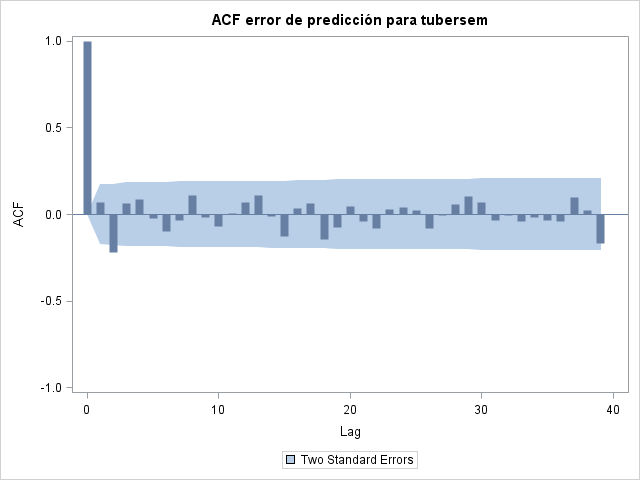
\includegraphics[width=0.75\textwidth]{ACF_ADD}
        \caption{Gráfico de autocorrelaciones (correlograma) para los residuales del modelo de \emph{Winter Aditivo} sobre el conjunto de datos \texttt{EJ2.SEMANAL4}}
        \label{img:b_winter_additive_residuals_correlogram}
      \end{figure}

      \paragraph{}
      Siguiendo la línea de lo comentado para el ACF del seasonal, vemos que para el retardo 2 de nuevo vuelve a ser una autocorrelación muy alta que indicará que solo se validará si no encontramos uno mejor. Para las autocorrelaciones para los periodos estacionales no se observa valores altos.

      \begin{figure}[htb!]
        \centering
        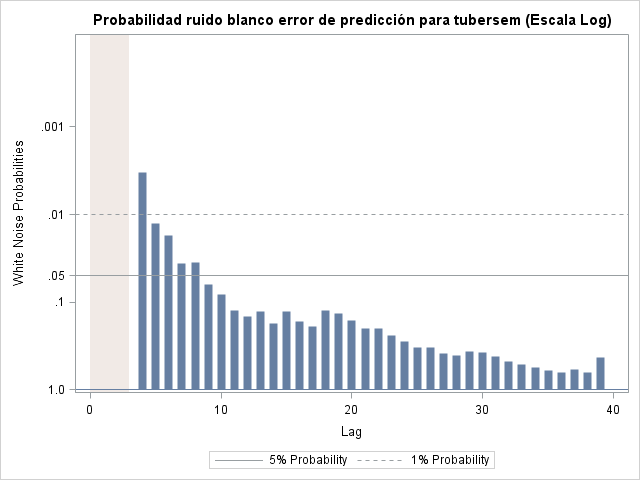
\includegraphics[width=0.75\textwidth]{WN_ADD}
        \caption{Gráfico sobre el contraste de ruido blanco para los residuales del modelo de \emph{Winter Aditivo} sobre el conjunto de datos \texttt{EJ2.SEMANAL4}}
        \label{img:b_winter_additive_test_white_noise}
      \end{figure}

      \paragraph{}
      Siguiendo el análisis de este modelo para determinar si es un modelo con ruido blanco o no, vemos en dicha gráfica que de nuevo se rechaza para los primeros retardos y por tanto no será ruido blanco, algo indeseable para validar el modelo.

      \paragraph{}
      Por último analizaremos el modelo Winter multiplicativo.

    \subsection{Winter Multiplicativo}

      \paragraph{}
      [TODO]

      \begin{listing}[htb!]
        \centering
        \inputminted{SAS}{./res/code/b-01-esm-wintermul.sas}
        \caption{Código fuente para el ajuste de un modelo de \emph{Winter Multiplicativo} sobre el conjunto de datos \texttt{EJ2.SEMANAL4}}
        \label{code:b_winter_multiplicative_esm}
      \end{listing}

      \paragraph{}
      [TODO]

      \paragraph{}
      Para comenzar se adjunta la tabla de significancia:

      \begin{table}[htb!]
        \centering
        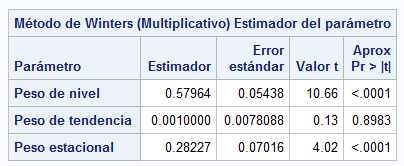
\includegraphics[width=0.75\textwidth]{TablaMUL}
        \caption{Significancia para el modelo de \emph{Winter Multiplicativo} sobre el conjunto de datos \texttt{EJ2.SEMANAL4}}
        \label{table:b_winter_multiplicative_significance}
      \end{table}

      \paragraph{}
      Observamos en la tabla anterior , que en este caso si se rechaza para la constante de suavizado estacional con un pvalor$ <0.001$ y para el nivel. Sin embargo, para la constantes de suavizado para la tendencia , no se rechaza la hipótesis de $\alpha_2 =0$, por lo que concluimos no será adecuado suavizar dicha componente. Vemos que su estimador es próximo a cero, por lo que será conveniente diferenciar o utilizar modelos ARIMA.

      \begin{figure}[htb!]
        \centering
        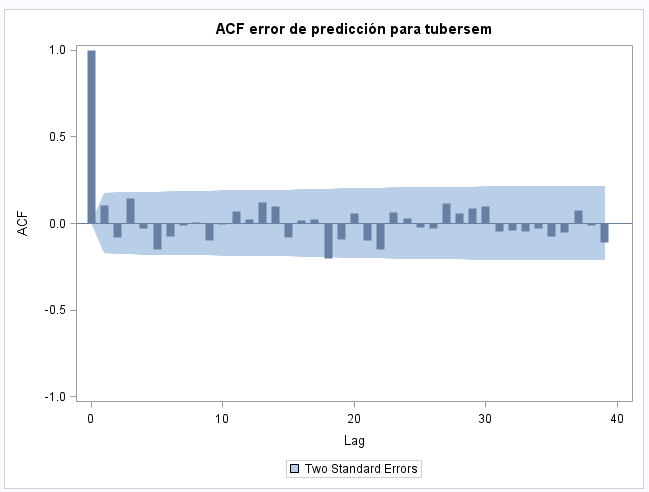
\includegraphics[width=0.75\textwidth]{ACF_MUL}
        \caption{Gráfico de autocorrelaciones (correlograma) para los residuales del modelo de \emph{Winter Multiplicativo} sobre el conjunto de datos \texttt{EJ2.SEMANAL4}}
        \label{img:b_winter_multiplicative_residuals_correlogram}
      \end{figure}

      \paragraph{}
      En el gráfico adjunto anteriormente, vemos como los primeros retardos son ligeramente menores a los de los otros modelos, donde en ningún caso sobrepasan las bandas. Los retardos para los periodos no son muy altos, quizás solo la autocorrelación 18 pero no es tan influyente en el ajuste.

      \begin{figure}[htb!]
        \centering
        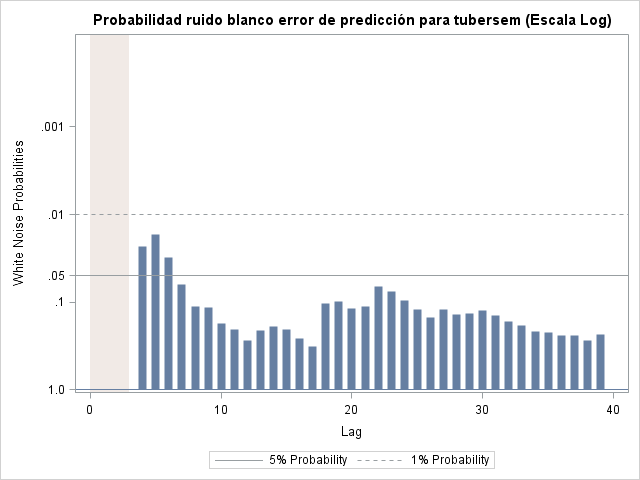
\includegraphics[width=0.75\textwidth]{WN_MUL}
        \caption{Gráfico sobre el contraste de ruido blanco para los residuales del modelo de \emph{Winter Multiplicativo} sobre el conjunto de datos \texttt{EJ2.SEMANAL4}}
        \label{img:b_winter_multplicative_test_white_noise}
      \end{figure}

      \paragraph{}
      Para finalizar, vemos el gráfico WN para contrastar si los residuales del modelo son ruido blanco. En este caso, diferenciandose ligeramente con los modelos anteriores, vemos que para $\alpha$ del 0.01 no se rechaza ninguno y solo 3 para $\alpha$ 0.05.

      \paragraph{}
      Por último compararemos SSE de cada modelo a modo de información adicional:

      \begin{table}[htb!]
        \centering
        \begin{tabular}{|l|r|}
            \hline
            \bfseries Modelo & $SSE$
            \csvreader[head to column names]{res/data/sse.csv}{}
            {\\\hline\MODEL & \SSE}
            \\ \hline
        \end{tabular}
        \caption{Relación entre los modelos ajustados y su \emph{Suma de Cuadrados del Error}.}
        \label{table:sse_comparative}
      \end{table}

    \paragraph{}
    [TODO ]

  \section{Elegir el modelo que se considere más apropiado entre los tres del apartado \ref{sec:b} y con ese modelo dar las predicciones para las próximas $6$ observaciones. Justificar la elección del modelo.}
  \label{sec:c}

    \paragraph{}
    [TODO]

    \begin{listing}[htb!]
      \centering
      \inputminted{SAS}{./res/code/c-01-prediction.sas}
      \caption{Código fuente para el ajuste y predicción de las $5$ observaciones siguientes de un modelo de \emph{Winter Multiplicativo} sobre el conjunto de datos \texttt{EJ2.SEMANAL4}}
      \label{code:winter_multiplicative_prediction}
    \end{listing}

    \paragraph{}
    [TODO]

    \paragraph{}
    Tras realizar un exhaustivo análisis en el apartado b, de los 3 modelos de suavizado exponencial, hemos considerado que el mejor modelo es el multiplicativo de Winter.
    Esta eleccion la hemos concluido por los motivos mencionados anteriormente :

    \begin{itemize}
      \item Pvalores de la \autoref{table:b_winter_multiplicative_significance} (Constante de Suavizado Estacional Significativa)
      \item Gráfica ACF de la \autoref{img:b_winter_multiplicative_residuals_correlogram} (Autocorrelaciones menores que otro modelos)
      \item Grafica WN de la \autoref{img:b_winter_multplicative_test_white_noise} (Retardos con menor probabilidad menor de ser ruido blanco)
    \end{itemize}

    \paragraph{}
    Por último, obtenemos las predicciones para las seis siguientes observaciones.

    \begin{table}[htb!]
      \centering
      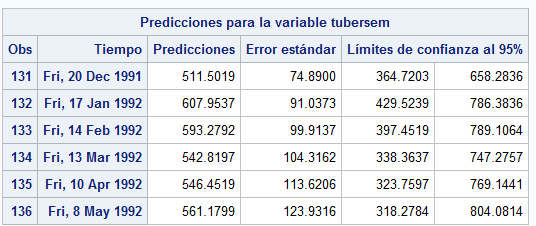
\includegraphics[width=0.75\textwidth]{PredC}
      \caption{Predicciones.Modelo Multiplicativo}
      \label{}
    \end{table}

    \paragraph{}
    [TODO]

  \section{Utilizando en el ajuste solamente los datos hasta el final de $1990$ que no incluyan ningún caso de $1991$, calcular los errores de predicción para el año $1991$ y su correspondiente $SSE_p$ (suma de $s$ errores al cuadrado correspondientes a predicciones $\{1, 2, ..., s\}$ pasos hacia adelante) para los tres modelos del apartado \ref{sec:b}. Comentar si la elección hecha en el apartado \ref{sec:c} está de acuerdo con los resultados obtenidos en este caso al comparar la capacidad de predicción de los distintos modelos para el año $1991$. Adjuntad el programa con el lenguaje control que hayáis utilizado en este apartado.}
  \label{sec:d}

    \paragraph{}
    [TODO]

    \paragraph{}
    Para calcular el $SSE_p$, primero explicaremos resumidamente que és y en que basa. El $SSE_p$ es el cálculo de una medida para comparar la capacidad de predicción de un modelo de series temporales.
    Se trata de predecir observaciones de una serie estacional de periodo s, para
    medir la capacidad de predicción de un modelo ajustado a dicha serie.

    \paragraph{}
    Si se dispone de n observaciones en total, $x_1,x_2...x_n$ se reservan las últimas k observaciones, donde k es un múltiplo de s. Para el ajuste se utilizan m observaciones ($m = n - k$) y la medida se obtiene sumando los cuadrados de los residuales $\{1, 2, ..., k\}$ pasos hacia adelante. Esto se define en la \autoref{eq:sse_p}.

    \begin{equation}
    \label{eq:sse_p}
      \begin{split}
        SSE_p
        &= \sum_{j = 1} ^ k (x_{m + j} - x_{m}(j)) ^ 2 \\
        &= \sum_{j = 1} ^ k e_m(j) ^ 2 \\
        &= e_m(1) ^ 2 + e_m(2) ^ 2 + ... + e_m(k) ^ 2
      \end{split}
    \end{equation}

    \begin{table}[htb!]
      \centering
      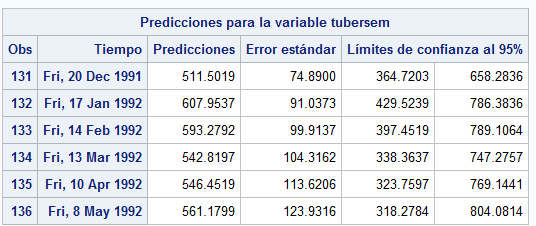
\includegraphics[width=0.75\textwidth]{PredC}
      \caption{Predicciones.Modelo Multiplicativo}
      \label{}
    \end{table}

    \paragraph{}
    A continuación, se adjunta una tabla con los valores predichos, los errores de predicción, y el SSE acumulado para cada observación de las 13 predichas, traduciéndose finalmente en el SSEp en la observacion 130.

    \begin{table}[htb!]
      \centering
      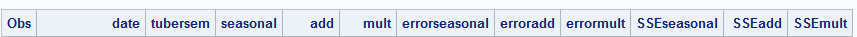
\includegraphics[width=\textwidth]{cabecera}
      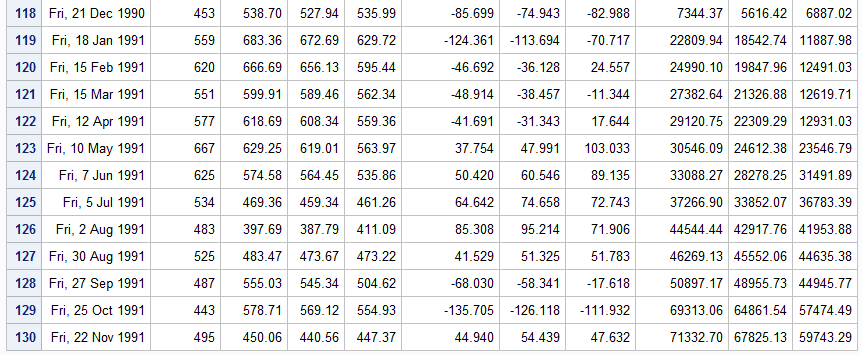
\includegraphics[width=\textwidth]{Errores}
      \caption{Errores Modelos. Seasonal Add Mul [TODO]}
      \label{}
    \end{table}

    \paragraph{}
    En la tabla siguiente se adjunta la capacidad de predicción para los 3 modelos, donde observamos que el que mejor predirá
    es el modelo de Winter multiplicativo con un menor SSEp de 59743.29.

    \begin{table}[htb!]
      \centering
      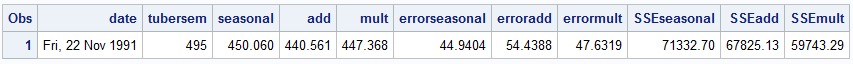
\includegraphics[width=0.75\textwidth]{SSEP_D}
      \caption{Predicciones SSEP. Seasonal Ad Mul}
      \label{}
    \end{table}

    \paragraph{}
    [TODO]

    \begin{listing}[htb!]
      \centering
      \inputminted{SAS}{./res/code/d-01-cross-validation.sas}
      \caption{[TODO]}
      \label{code:d_cross_validation}
    \end{listing}

    \paragraph{}
    [TODO]

    \begin{listing}[htb!]
      \centering
      \inputminted{SAS}{./res/code/d-02-prediction-error-esm-seasonal.sas}
      \caption{[TODO]}
      \label{code:d_prediction_error_esm_seasonal}
    \end{listing}

    \paragraph{}
    [TODO]

    \begin{listing}[htb!]
      \centering
      \inputminted{SAS}{./res/code/d-02-prediction-error-esm-winteradd.sas}
      \caption{[TODO]}
      \label{code:d_prediction_error_esm_winteradd}
    \end{listing}

    \paragraph{}
    [TODO]

    \begin{listing}[htb!]
      \centering
      \inputminted{SAS}{./res/code/d-02-prediction-error-esm-wintermul.sas}
      \caption{[TODO]}
      \label{code:d_prediction_error_esm_wintermul}
    \end{listing}

    \paragraph{}
    [TODO]

    \begin{listing}[htb!]
      \centering
      \inputminted{SAS}{./res/code/d-03-error-summary.sas}
      \caption{[TODO]}
      \label{code:d_summary_error}
    \end{listing}

    \paragraph{}
    [TODO]

  \section{Obtener con el \texttt{proc forecast} de \emph{SAS} el $SSE_p$ para el modelo de \emph{Winter Multiplicativo} con las mismas constantes de suavizado y los valores iniciales de los parámetros lo más próximos posible a los obtenidos en el apartado \ref{sec:d} con el \texttt{proc esm} para este modelo. Adjuntar el programa con el lenguaje control que hayáis utilizado para obtenerlo.}
  \label{sec:e}

    \paragraph{}
    [TODO]

    \paragraph{}
    Esta primera tabla se ha obtenido de la misma manera que en el apartado anterior probando a variar  el  atributo NSSTART que finalmente se realizo para 2 obteniendo un SSEp de 62801.35 que es muy semejante al obtenido con \textit{proc esm}.

    \begin{table}[htb!]
      \centering
      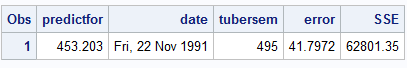
\includegraphics[width=0.7\textwidth]{TablaSSEPFOR}
      \caption{Predicciones SSEP Forecast. Multiplicativo}
      \label{}
    \end{table}

    \paragraph{}
    Hay otra manera en la que no hace falta ir modificando el valor en NSStart.

    \begin{table}[htb!]
      \centering
      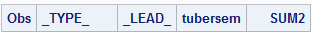
\includegraphics[width=0.5\textwidth]{cabecera2}
      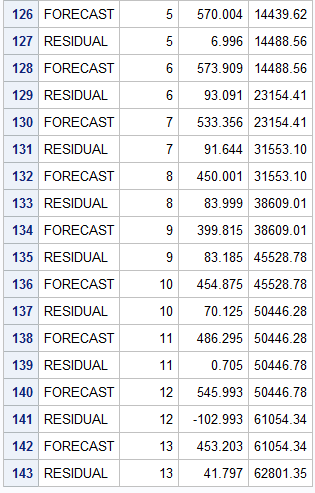
\includegraphics[width=0.5\textwidth]{SSEPFOR}
      \caption{[TODO]}
      \label{}
    \end{table}

    \paragraph{}
    [TODO]

    \begin{listing}[htb!]
      \centering
      \inputminted{SAS}{./res/code/e-prediction-forecast-method-1.sas}
      \caption{Código Fuente para cálculo del error de predicción $SSE_p$ mediante el \texttt{proc forecast} por el primer método.}
      \label{code:prediction_forecast_method_2}
    \end{listing}

    \paragraph{}
    [TODO]

    \begin{listing}[htb!]
      \centering
      \inputminted{SAS}{./res/code/e-prediction-forecast-method-2.sas}
      \caption{Código Fuente para cálculo del error de predicción $SSE_p$ mediante el \texttt{proc forecast} por el segundo método.}
      \label{code:prediction_forecast_method_2}
    \end{listing}

    \paragraph{}
    [TODO]

  \section{Ajustar un modelo para la serie $\{ Xt \}$ con el módulo \texttt{Time Series Forecasting System} de \emph{SAS} razonando porqué se ha elegido. Utilizar el modelo elegido para predecir valores futuros de esta serie y establecer la comparación con los seis valores obtenidos en el apartado \ref{sec:c} junto con sus bandas de predicción.}
  \label{sec:f}

    \paragraph{}
    [TODO]

\end{document}
